\chapter{Design artefacts}
\label{appendix5-design-artefacts}
\graphicspath{{Appendix5/Figs/}{Appendix5/Figs/}}

In this appendix, design artefacts are displayed that were created during the 10 sprints of the project to create the next version of IDUN’s NIP.

\section*{Console web app wireframes}

The following wireframes are the result of user interviews and internal group discussions. The following figures show the future version of the Console web application for IDUN, which is scheduled for release in early 2023.

\begin{figure}[!ht]
  \centering
  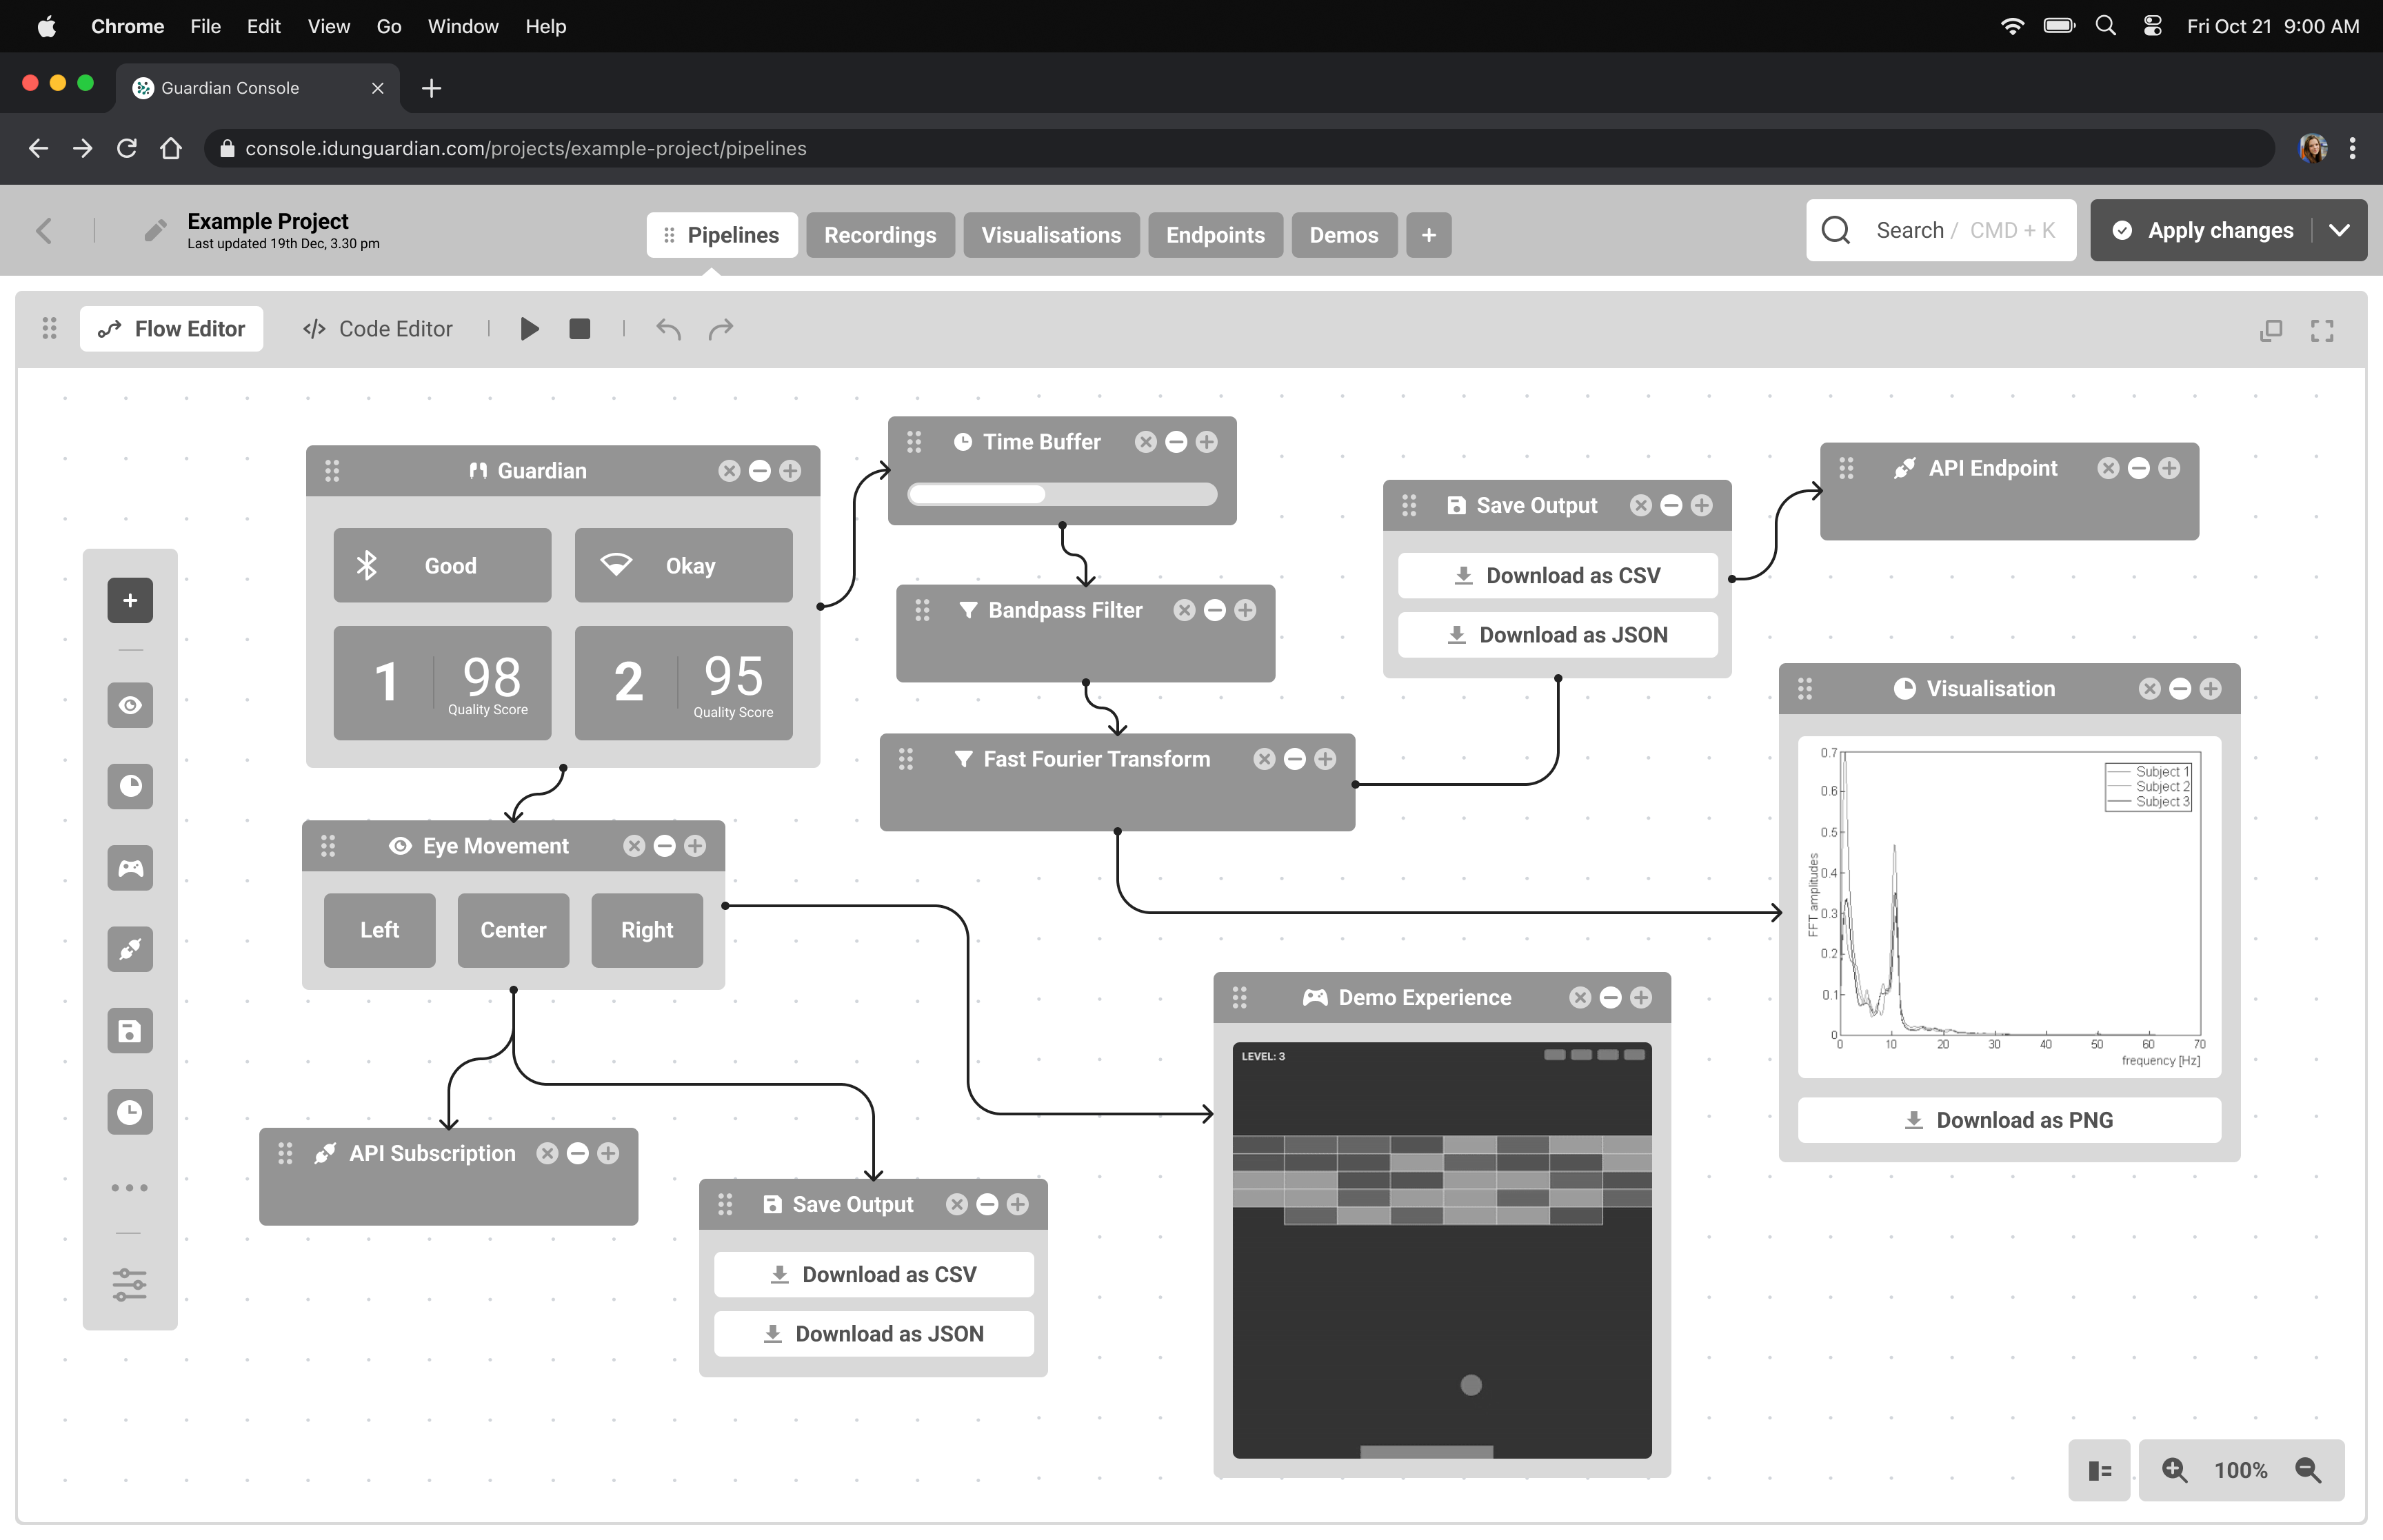
\includegraphics[width=\linewidth]{new-console_start.png}
  \caption{Screenshot No. 1 of an exploratory draft for the web version of the Console to be released in early 2023.}
  \label{fig:console-wireframe-001}
\end{figure}

\autoref{fig:console-wireframe-001} demonstrates the ability to create deployable neural signal processing pipelines via a drag-and-drop no-code editor.

\begin{figure}[!ht]
  \centering
  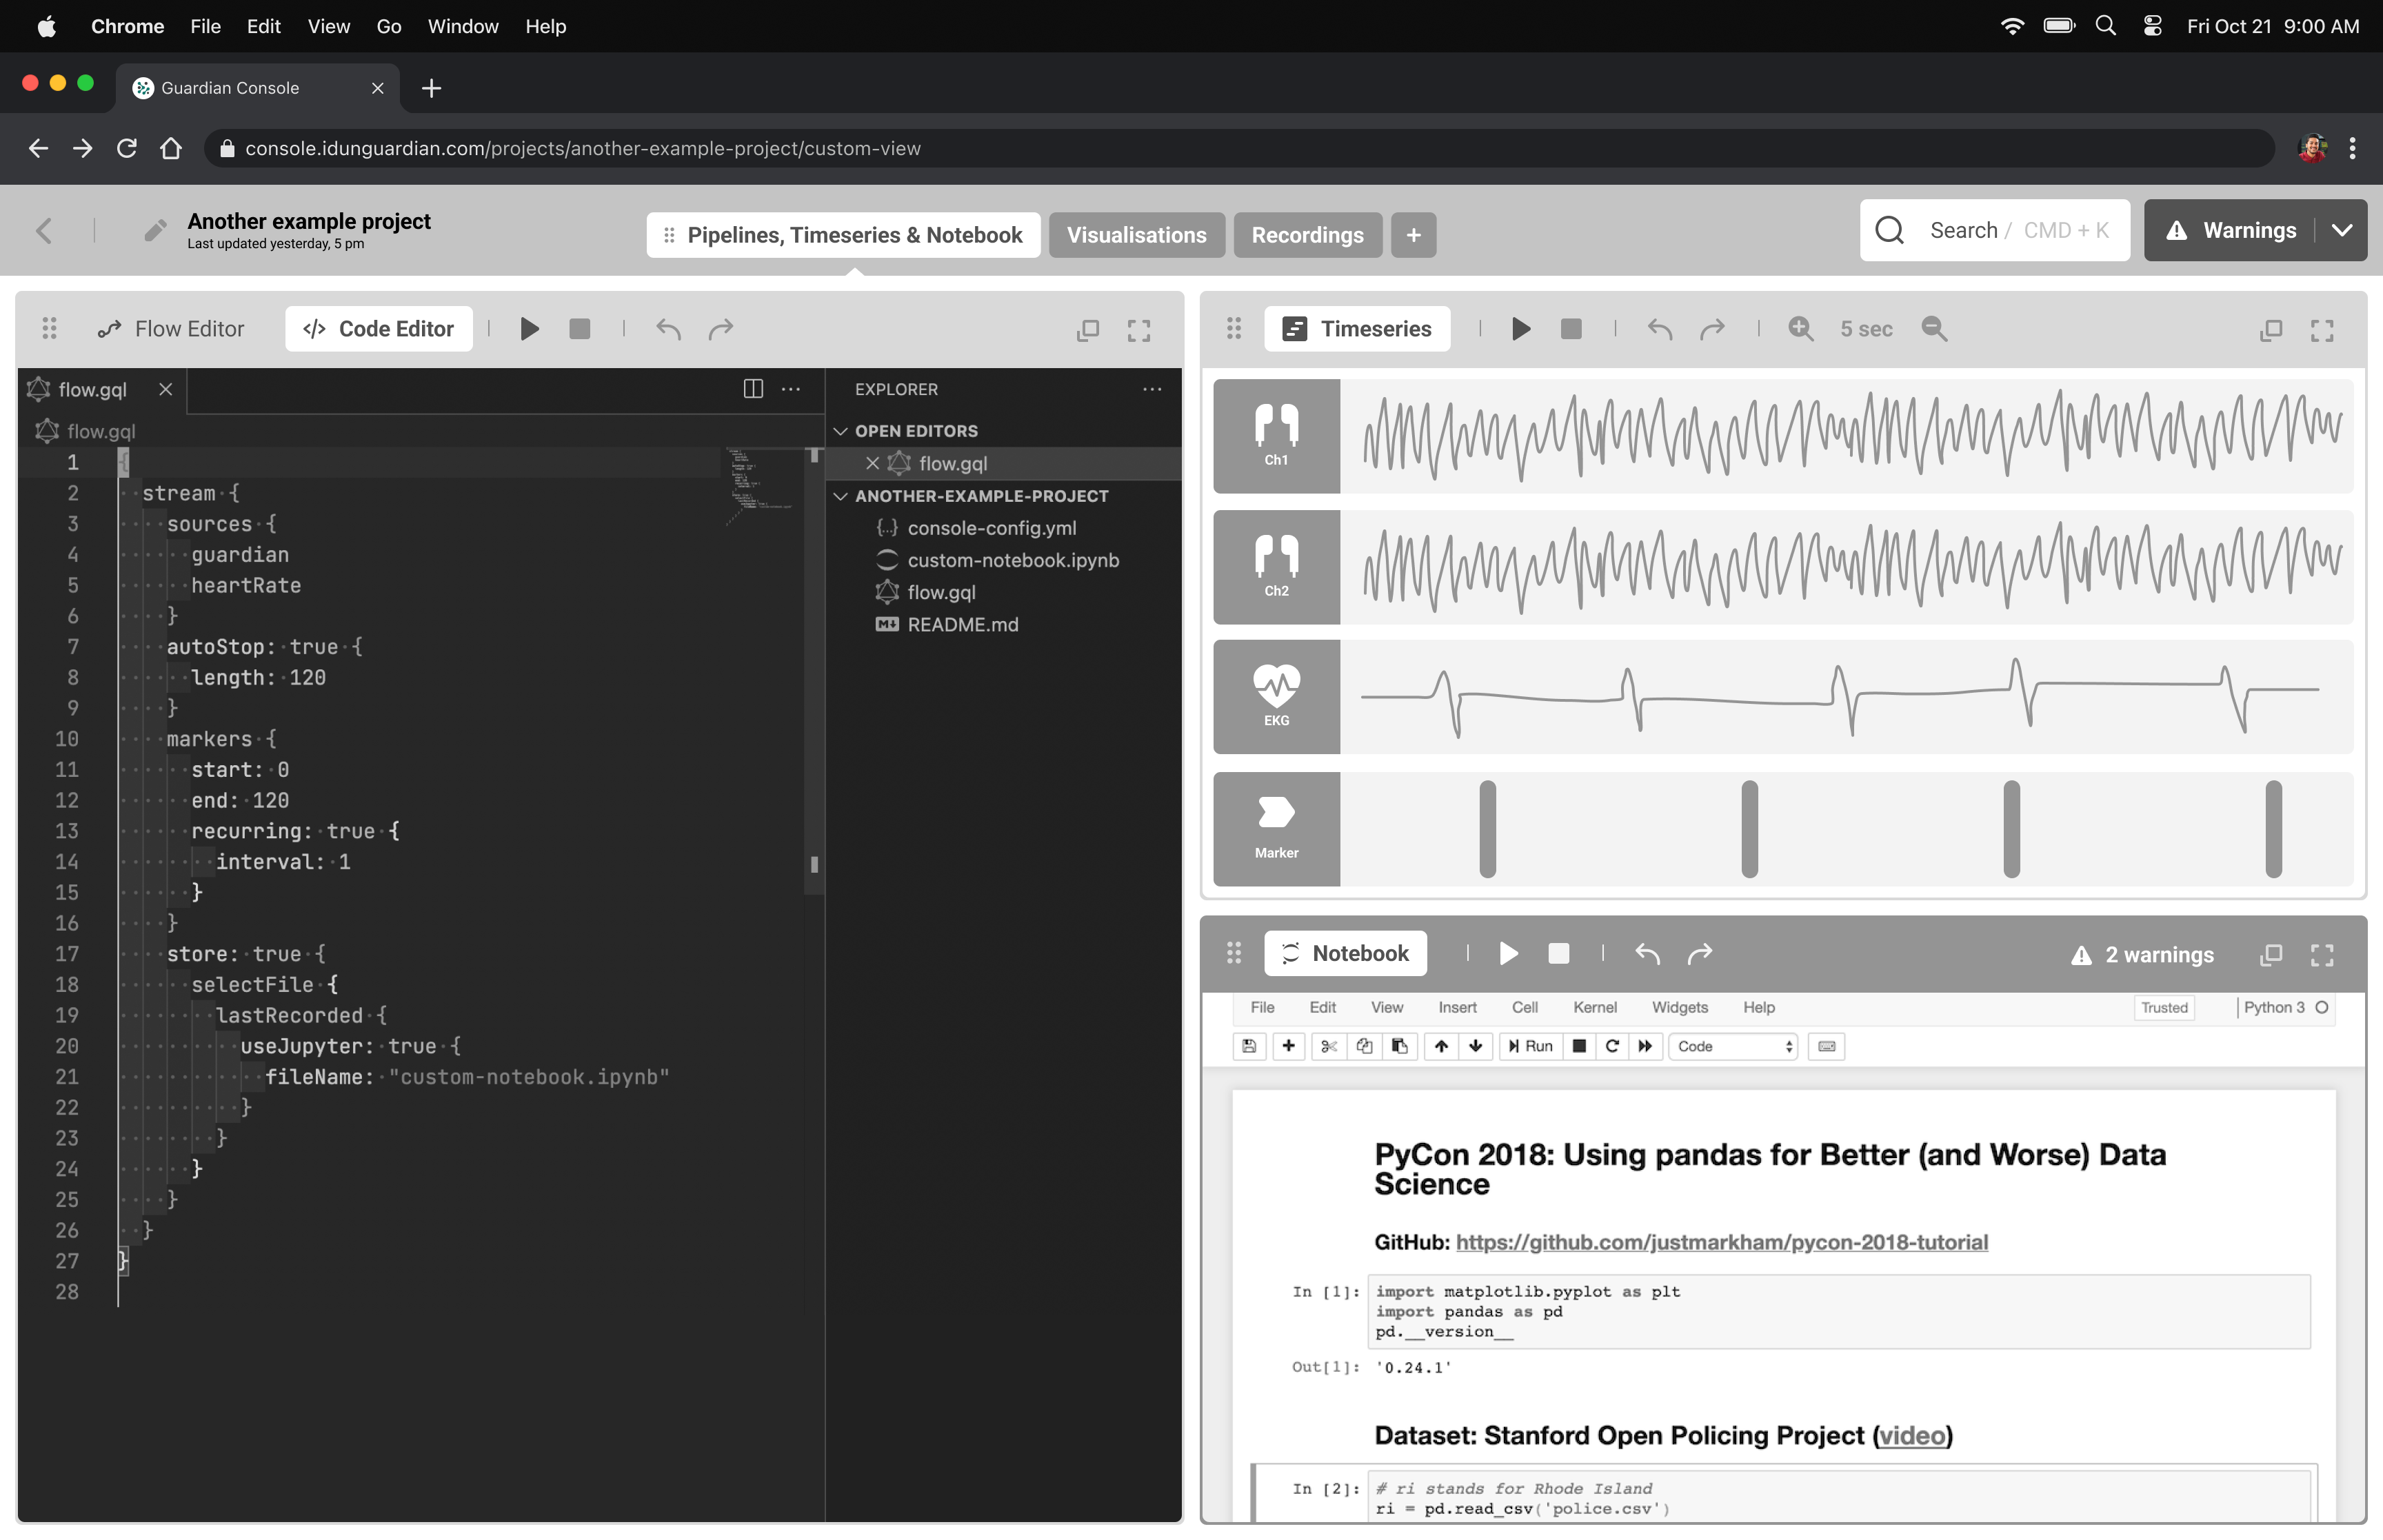
\includegraphics[width=\linewidth]{new-console_code-view.png}
  \caption{Screenshot No. 2 of an exploratory draft for the web version of the Console to be released in early 2023.}
  \label{fig:console-wireframe-002}
\end{figure}

\autoref{fig:console-wireframe-002} shows how, in addition to the visual no-code editor, advanced users, such as the Evan persona, can also work directly on code generated via the IDUN SDK.

\section*{Authentication web app wireframes}

The following wireframes are the result of internal group discussions, expert interviews and, in particular, the findings of IDUN Technologies’ neuroethics advisory board in order to protect user privacy and restrict access to the generated insights and raw EEG data. The following figures show the future version of an authentication web app for IDUN, scheduled for release in early 2023.

\begin{figure}[ht]
  \centering
  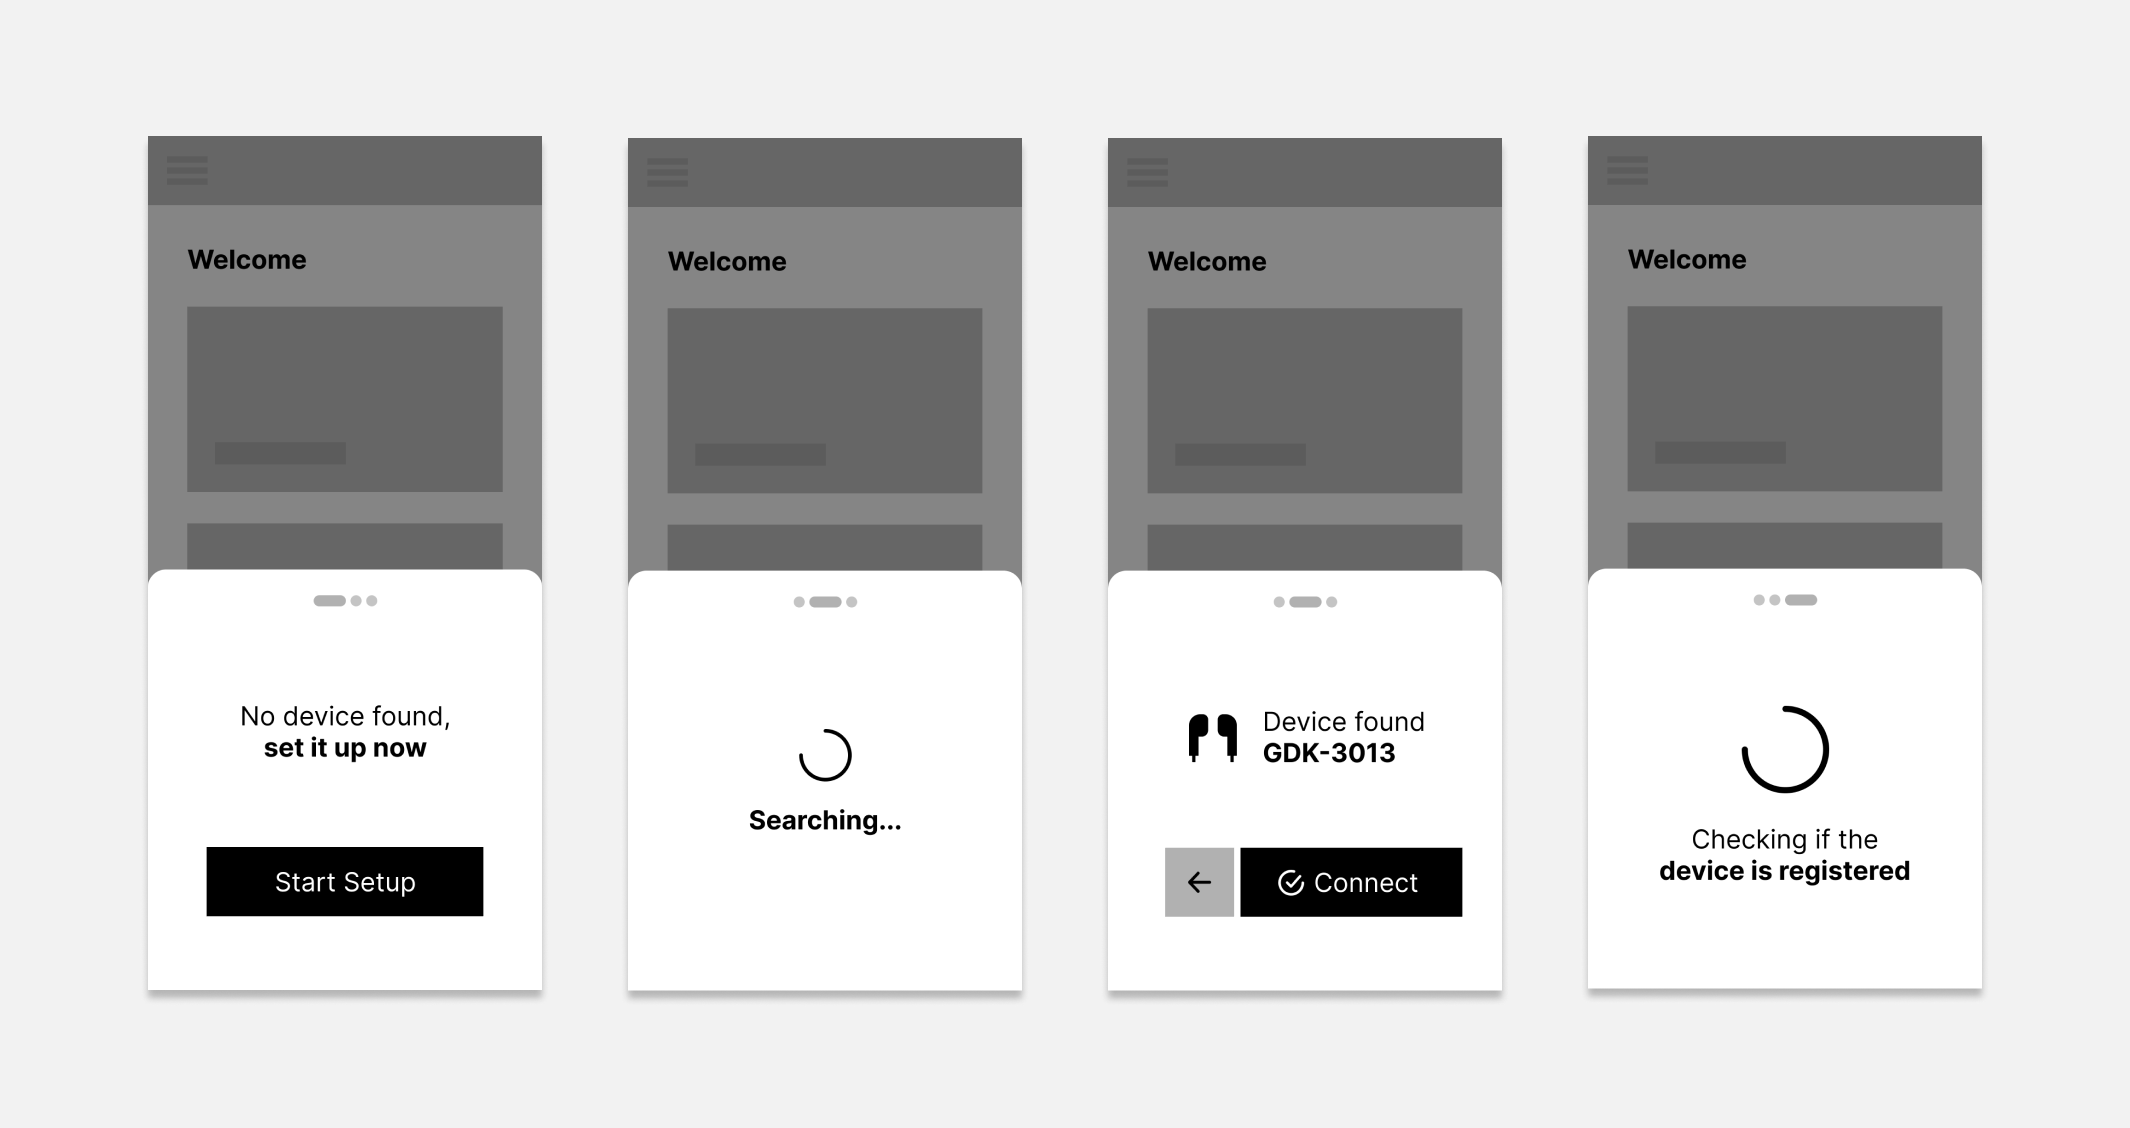
\includegraphics[width=\linewidth]{design_artefacts_001.png}
  \caption{Screenshot No. 1 of an exploratory wireframe draft for the version of the authentication web app to be released in early 2023.}
  \label{fig:auth-wireframe-001}
\end{figure}

\autoref{fig:auth-wireframe-001} shows how a slide-over would look in the third-party app if no device from IDUN is connected to, for example, a smartphone. After searching for BLE devices with certain characteristics, the nearest device is displayed with the option to connect to it. After this process, the SDK integrated in the third-party app checks whether this device is registered in the IDUN cloud with this identifier.

\begin{figure}[ht]
  \centering
  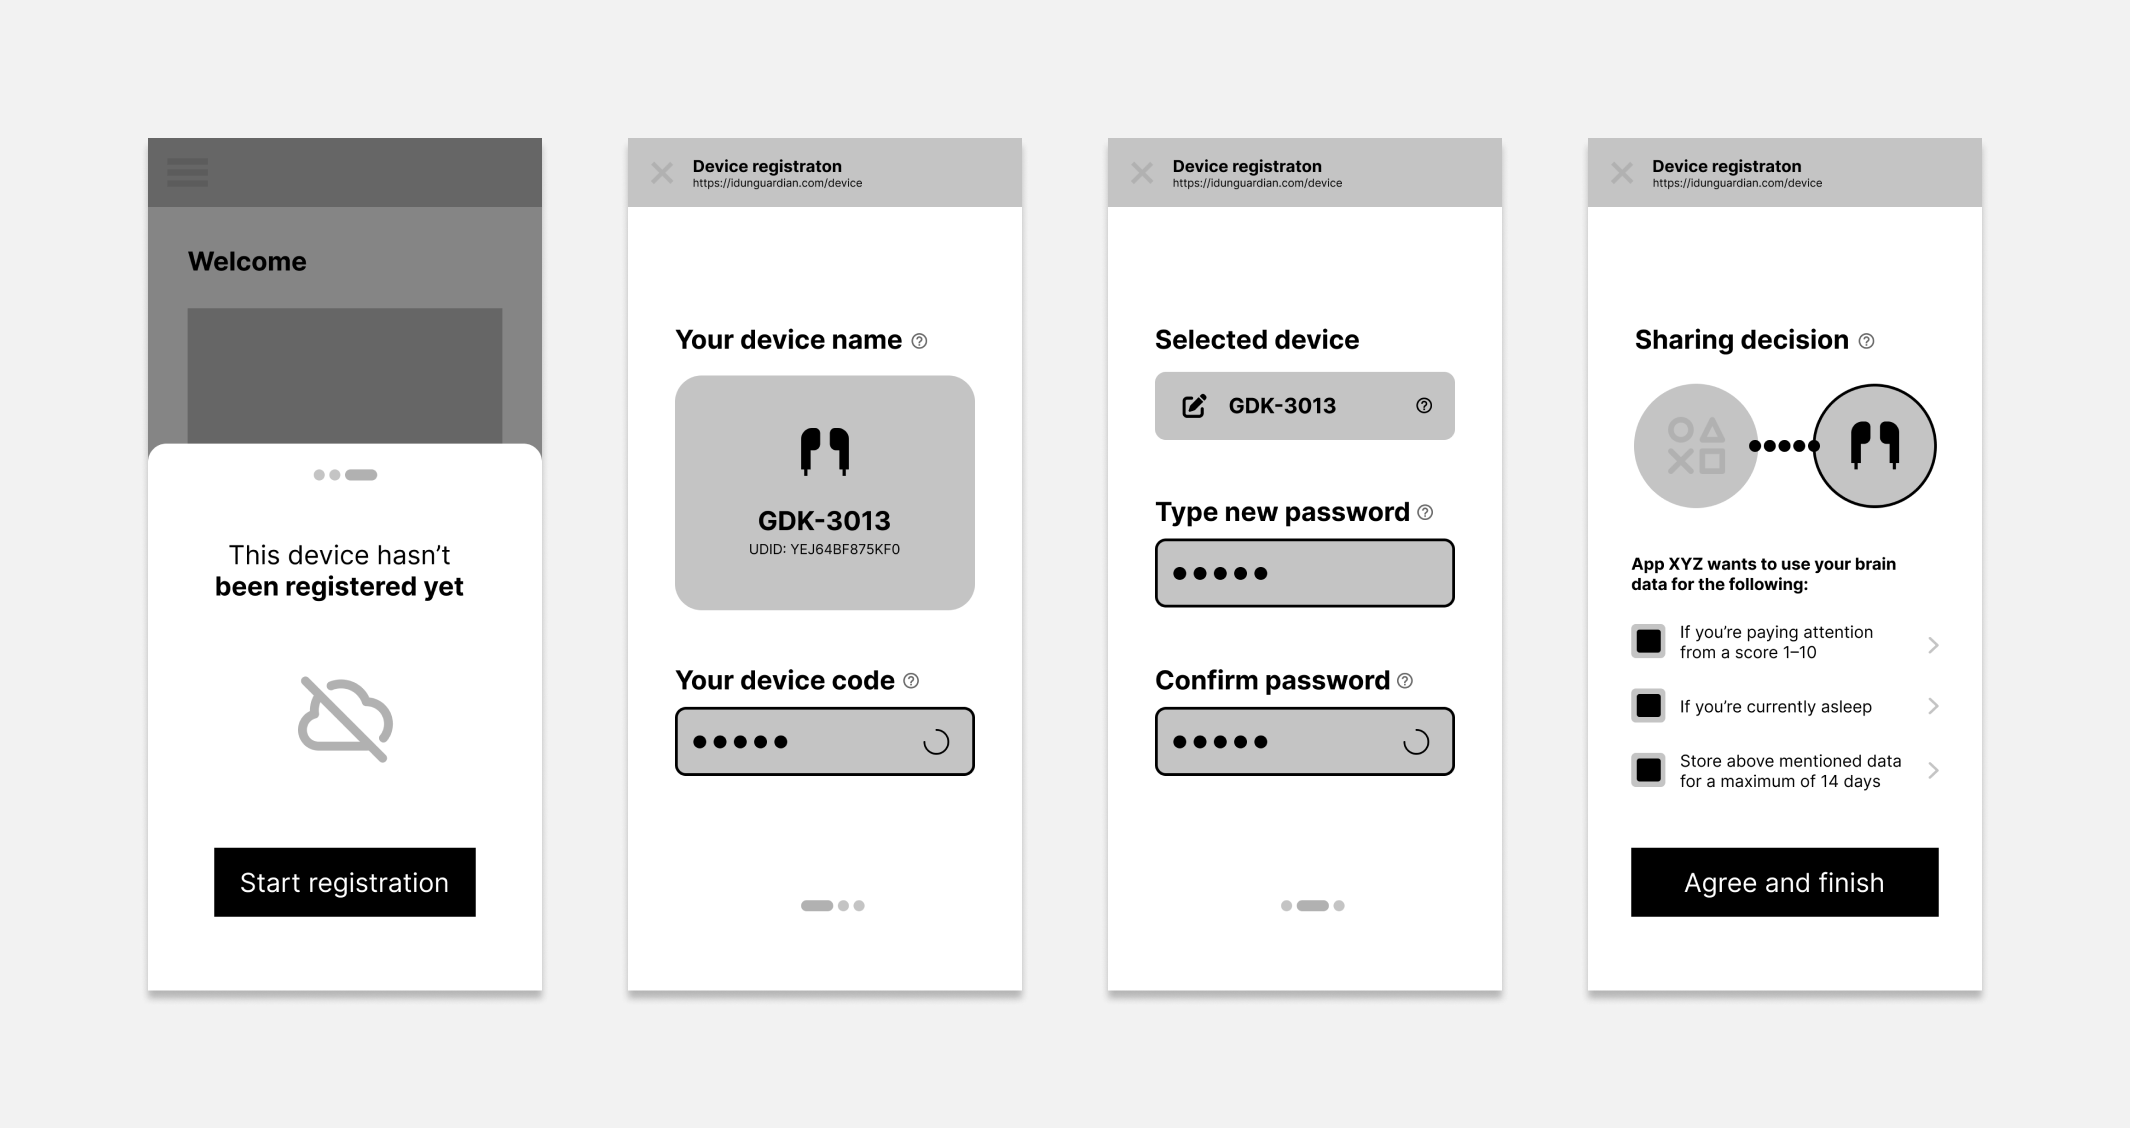
\includegraphics[width=\linewidth]{design_artefacts_002.png}
  \caption{Screenshot No. 2 of an exploratory wireframe draft for the version of the authentication web app to be released in early 2023.}
  \label{fig:auth-wireframe-002}
\end{figure}

\autoref{fig:auth-wireframe-002} shows how the process would look if IDUN’s device is not yet registered in the cloud, for example, the opt-in for the specific third-party app in this example is not yet granted. Therefore, the user must authenticate with a device password (which they must reset the first time they use it) and then select specific options to which they agree.
